\documentclass[11pt,openright,a4paper]{report}
%%
%% This document template assumes you will use pdflatex.  If you are using
%% latex and dvipdfm to translate to pdf, insert dvipdfm into the options.
%%

%%
%% Package includes to provide the basic style
%%
\usepackage{harvard}    % Uses harvard style referencing
\usepackage{graphicx}   % Permits import of various graphics formats
\usepackage{hyperref}   % Provides hyperlinks to sections automatically
\usepackage{pdflscape}  % Provides landscape mode for end code listings
\usepackage{multicol}   % Provides ability to split output into columns
\usepackage{listings}   % Provides styled code listings


%%
%% Set some page size changes from the standard article class
%%
\usepackage{calc}
\setlength{\parskip}{6pt}
\setlength{\parindent}{0pt}
\addtolength{\hoffset}{-0.5cm}
\addtolength{\textwidth}{2.5cm}


%%
%% Format definitions for the style
%%
\bibliographystyle{agsm}  %{alpha}
\citationstyle{dcu}
\pagestyle{headings}
\fussy


%%
%% Definitions to provide layout in the dissertation title pages
%%
\newenvironment{spaced}[1]
  {\begin{minipage}[c]{\textwidth}\vspace{#1}}
  {\end{minipage}}


\newenvironment{centrespaced}[2]
  {\begin{center}\begin{minipage}[c]{#1}\vspace{#2}}
  {\end{minipage}\end{center}}


\newcommand{\declaration}[2]{
  \thispagestyle{empty}
  \begin{spaced}{4em}
    \begin{center}
      \LARGE\textbf{#1}
    \end{center}
  \end{spaced}
  \begin{spaced}{3em}
    \begin{center}
      Submitted by: #2
    \end{center}
  \end{spaced}
  \begin{spaced}{5em}
    \section*{COPYRIGHT}

    Attention is drawn to the fact that copyright of this dissertation rests
    with its author. The Intellectual Property Rights of the products
    produced as part of the project belong to the author unless otherwise specified
    below, in accordance with the University of Bath's policy on intellectual property 
   (see http://www.bath.ac.uk/ordinances/22.pdf).

    This copy of the dissertation has been supplied on condition that anyone
    who consults it is understood to recognise that its copyright rests with its
    author and that no quotation from the dissertation and no information
    derived from it may be published without the prior written consent of
    the author.

    \section*{Declaration}
    This dissertation is submitted to the University of Bath in accordance
    with the requirements of the degree of Bachelor of Science in the
    Department of Computer Science. No portion of the work in this dissertation
    has been submitted in support of an application for any other degree
    or qualification of this or any other university or institution of learning.
    Except where specifically acknowledged, it is the work of the author.
  \end{spaced}

  \begin{spaced}{5em}
    Signed:
  \end{spaced}
  }


\newcommand{\consultation}[1]{%
\thispagestyle{empty}
\begin{centrespaced}{0.8\textwidth}{0.4\textheight}
\ifnum #1 = 0
This dissertation may be made available for consultation within the
University Library and may be photocopied or lent to other libraries
for the purposes of consultation.
\else
This dissertation may not be consulted, photocopied or lent to other
libraries without the permission of the author for #1 
\ifnum #1 = 1
year
\else
years
\fi
from the date of submission of the dissertation.
\fi
\vspace{4em}

Signed:
\end{centrespaced}
}

%%
%% END OF DEFINITIONS
%%


\usepackage{pdfpages}
\usepackage[number=none]{glossary}

%% Configure these to your own personal details
\newcommand{\disstitle}{The potential of declarative programming languages to support
user interface programming: the case of ELM}
\newcommand{\authorname}{Simon Buist}
\newcommand{\degree}{Computer Science}
\newcommand{\submissiondate}{October 2013}

\title{Literature Review\\[1in]\disstitle}
\author{\authorname}
\date{Bachelor of Science in \degree\\The University of 
Bath\\\submissiondate}


%\makeglossary
%% Glossary of terms

%\glossary{
%	name={experiment},
%	description={at the heart of every experiment there's a good question. These
%	questions come from observation.}
%}

\begin{document}

\setcounter{page}{0}
\pagenumbering{roman}

\maketitle
\newpage

\tableofcontents
\newpage

\setcounter{page}{1}
\pagenumbering{arabic}

\chapter{A survey of relevant papers}

%Using the hypothesis you have developed or the project idea you have identified,
%you should use the reading to identify the major ideas and threads of
%development, relate work that has (perhaps) not previously been related, and
%thereby justify and refine your hypothesis / ideas. The Literature Review
%should "tell a story" that identifies the development and blossoming of your
%ideas as you conducted your literature search. It is worth repeating that it
%should not be merely a catalogue of the items you have read. The precise form
%of literature you will need to examine will vary depending upon the nature of
%your project. Highly research-related projects will invariably tend to draw upon
%a range of published papers from academic journals or conference proceedings,
%perhaps utilising a few key texts. The Literature Survey will start with an
%identification of the problem area and will use the Literature Review to
%identify previous work completed in the area and the major results. It will, of
%necessity, have to pull together a lot of small findings to paint a picture of
%the recent progress made within the area. It will lead towards an identification
%of key open questions that relate to your hypotheses and will highlight the
%evidence that your hypotheses are based upon. The Survey will normally culminate
%in the presentation of your hypothesis and an identification of the
%contributions to knowledge that you hope your work will make.
%
%The major ideas and threads of development
%
%Work that has perhaps not previously been related
%
%Refining hypothesis / ideas.

\section{Introduction to the problem area}

Spending half an hour making a mind-map, starting with the word ``Elm'', I get the following terms:

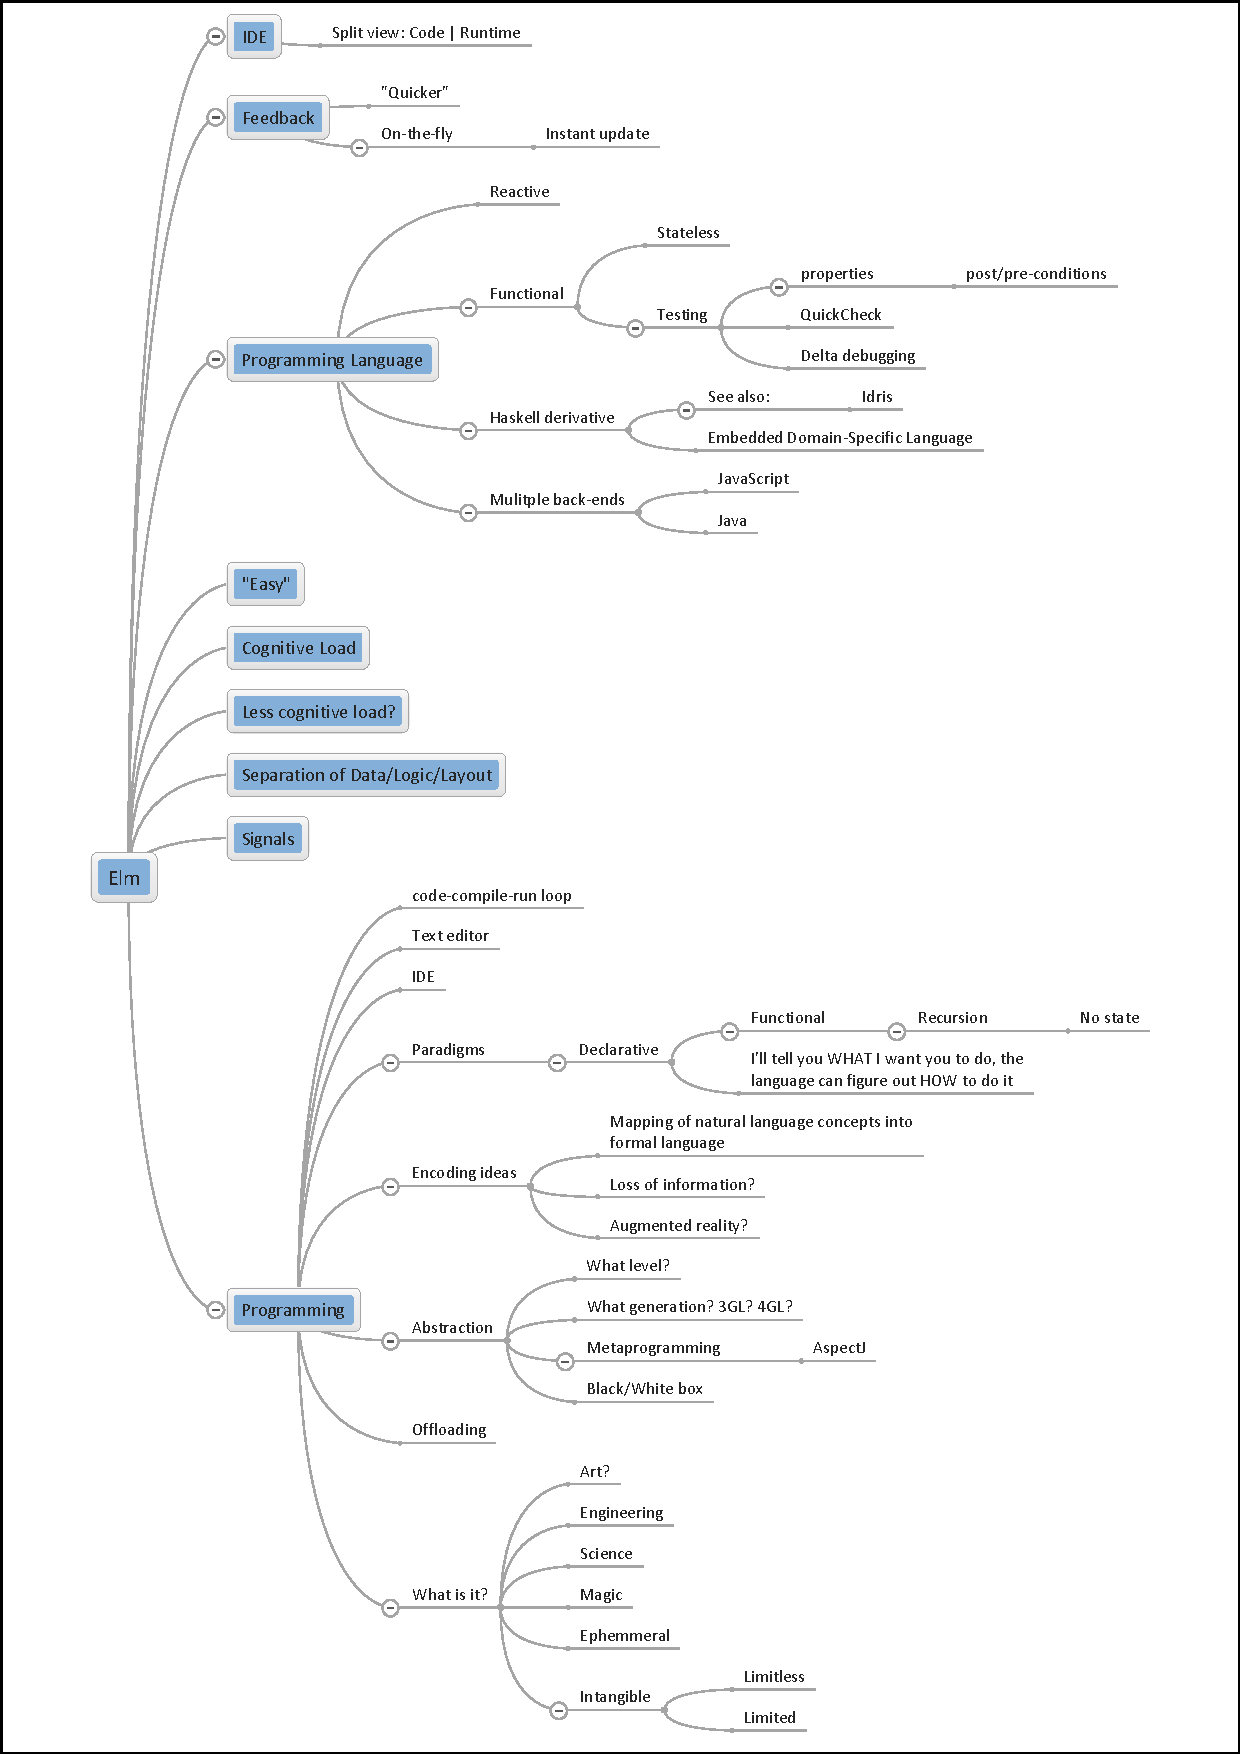
\includepdf[scale=0.65,pages=1,pagecommand=\subsection{Elm mind-map}\label{pdf:mindmap}]{mindmap.pdf}

In list form, with added terms:

\begin{itemize}
	\item Signals
	\begin{itemize}
		\item Impure
		\item Time
		\item Input/Output
		\item History -- Past \& Future
		\item Data model
	\end{itemize}
	\item ``Natural'' Separation of Data model/Logic/Layout
	\item Less cognitive load?
	\item ``Easy''
	\begin{itemize}
		\item Professed to be ``easy'' by the creator!
		\item What does it mean to be ``easy''?
		\item Operationalisation
		\item Self-reporting
	\end{itemize}
	\item Programming Language
	\begin{itemize}
		\item Reactive
		\begin{itemize}
			\item ``Instant feedback''
			\item ``I/O-sensitive''
			\item Thrashing?
		\end{itemize}
		\item Functional
		\begin{itemize}
			\item Pure
			\item Testing
			\begin{itemize}
				\item properties
				\item QuickCheck
				\item Delta Debugging
			\end{itemize}
		\end{itemize}
		\item Haskell derivative
		\begin{itemize}
			\item Embedded Domain-specific Language
			\item See also: Idris
		\end{itemize}
		\item Multiple back-ends
		\begin{itemize}
			\item Javascript
			\item Java
			\item C
		\end{itemize}
	\end{itemize}
	\item Programming
	\begin{itemize}
		\item code-compile-run loop
		\begin{itemize}
			\item ``Programming blind''
			\item ``Slow feedback''
		\end{itemize}
		\item Text editor
		\item IDE
		\item Paradigms
		\begin{itemize}
			\item Declarative
			\item I'll tell you WHAT I want you to do, you
			      figure out HOW to do it
		\end{itemize}
		\item Encoding ideas
		\begin{itemize}
			\item Mapping of natural language concepts into formal language
			\item Loss of information?
			\item Augmented reality?
		\end{itemize}
		\item Abstraction
		\begin{itemize}
			\item What level?
			\item What generation? 3GL? 4GL?
			\item Metaprogramming e.g. AspectJ
			\item Black/White box
		\end{itemize}
		\item Cognitive offloading
		\item What is it?
		\begin{itemize}
			\item Art?
			\item Engineering?
			\item Science?
			\item Language?
			\item Mathematics?
			\item Ephemeral
			\item Intangible
			\item Limitless
			\item Limited
		\end{itemize}
	\end{itemize}
	\item IDE
	\begin{itemize}
		\item Split View: Code | Runtime
	\end{itemize}
	\item Feedback
	\begin{itemize}
		\item ``Instant-update''
		\item On-the-fly
	\end{itemize}
\end{itemize}

The problem area of user-interface programming, and more generally, the activity
of programming in a context such as a software engineering environment,
encompasses certain realms of interest. Through my survey of literature, my
research has
touched upon the above-mentioned terms, and I have discovered some thought-provoking
problems that exist in the field of programming. The concept of `Programming'
embodies other concepts -- art-forms, engineering processes, 
science, language, and mathematics, among others. To me, programming is a
creative endeavour unlike any other -- in which the programmer weilds materials
of no substance -- the code -- by manipulating symbols on a screen, which
represent states in the machine being used. There are so many programming
languages, and all languages (all that are Turing-complete) reduce to the same
language -- that of a Turing Machine. So, \textit{why do we have so many
programming languages?}. 

\textit{Beware of the Turing tar-pit in which everything is possible but nothing of
interest is easy.} \cite{PerlisTuringTarpit}

Different languages lend themselves to different ways of
thinking about problems. They may place emphasis on one feature, for example
list manipulation and hide others such as types. The language or programming
environment may make explicit the
effect of changes as they are encoded, as opposed to queuing up a block of
changes and the programmer having to initiate an update manually.

I would like to draw your attention in particular to the terms
\textbf{Abstraction},
\textbf{Cognitive offloading}, \textbf{Feedback}, \textbf{Loss of
information?}/\textbf{Augmented reality?}, \textbf{Thrashing}, and
\textbf{``Programming blind''}. These, at current, are my topics of interest,
and my literature review has up to this point been inextricably and heavily
influenced by this.

Under the umbrella quote of "Don't program blind" -- tools that help the programmer see what he's doing:

From: [Don't Learn to Code, Learn to Program -- But come back in 10 years](http://johnkurkowski.com/posts/dont-learn-to-code-learn-to-program-but-come-back-in-10-years/):

Quite a sad title really. And sad content. BUT it does link to some wise words
from Jeff Atwood, Peter Norvig ("Learn to program in 10 years!"), and has a
handful of links to different projects and a nice quote:

\textit{
    If builders built buildings the way programmers wrote programs, then the
    first woodpecker that came along would destroy civilization.
}
        – Gerald M. Weinberg, The Psychology of Computer Programming (1971)


[Out in the open: These Hackers want to give youSuperpowers](http://www.wired.com/wiredenterprise/2014/01/light-table/)

    “We consider programming a modern-day superpower. You can create something out of nothing, cure cancer, build billion-dollar companies,” he says. “We’re looking at how we can give that super power to everyone else.”
    
    The problem with coding, he says, is that you can’t see the results of your work until after you’re done. In that sense, programming is unlike almost every other craft. “When a chef adds an ingredient, he can smell it, he can taste it,” Granger says. “When an artist makes a stroke on a canvas, he can see it. But programming isn’t that way.”
    
    \textit{‘We consider programming a modern-day superpower. You can create
	    something out of nothing, cure cancer, build billion-dollar
    companies.’}
    
    — Chris Granger
    
    Programmers may spend hours or days working on code before they can make sure it actually works. “We have to play computer in our heads,” he says. “We write each line, imagine what it will do. You have to act like a computer. The problem with that is that we’re pretty crappy computers.” But Light Table seeks to bridge that gap.
    
    Light Table is an open source programming tool that lets programmers see the results of their code as their write it. It’s not an entirely new idea. In the mid-1960s, an educational tool called Logo gave programming students immediate feedback. More recently, languages like the kid friendly Scratch and artist friendly Processing have offered a kind of visual feedback, giving coders more insight into their programs as they’re written.
    
    But applying those ideas to professional software — complex applications with thousands or even millions of lines of code — is another matter. Light Table tackles such software by not only by displaying the results of the code you’re working on right now, but by showing how it relates to other parts of your software and how data flow from one chunk of code to another. It also weaves documentation throughout the code, while offering new ways to organize and visualize the code in any application.

    \textbf{Flow Based Programming}

* [NoFlo](http://noflojs.org/), [Flowhub.io](http://flowhub.io/)
* BOOK: [J. Paul Morrison](http://www.jpaulmorrison.com/fbp/) -- Flow Based Programming
* [Example of NoFlo implementation of Jekyll](https://github.com/the-grid/noflo-jekyll)

\section{What does it mean to be `easy to use?'}

In the process of surveying relevant (and sometimes irrelevant) literature to
this dissertation, recurring conceptual patterns were observed -- one particular instance
of this is that several authors seem to lay victim to the trap of claiming their
creation is ``easy to use'', ``better'', ``simpler than \(x\)'' without
providing any supportive evidence of this.

Perhaps these are incidents of `experimenter bias' -- where
the evaluator is naturally predisposed to a positive appraisal of their own
findings. One way to avoid this is to have one set of people perform the data
capture and another set perform the data analysis. Nevertheless, these patterns
emerge, and present numerous opportunities for experimentation and subsequent
evidence supporting or contradicting these claims. Experiments may see if the
same conclusions are reached as the above-mentioned authors, accounting for the
`evaluator effect'  \cite{Hertzum2001}.

Whether this particular route is taken for experimentation hinges on pilot
studies that will be conducted concurrently to the Literature Survey,
each inextricably shaping the other's direction of investigation and inquiry. 

The catalyst to this whole dissertation was a talk about the concept of a highly
reactive development environment -- where changes in the code result in
instantaneous updates to the runtime, `on-the-fly'. This was presented in  Bret
Victor's ``Inventing on Principle'' \cite{Victor2012a}. In his presentation Bret
makes several assertions about the `traditional' style of coding, one statement
of which is that ``most of the developer's time is spent looking at the code,
blindly without an immediate connection to the thing they're making''. He argues
that ``so much of creation is discovery, and you can't discover anything if you
can't see what you're doing'' -- alluding to his earlier statement that the
compile-run-debug cycle is much like this. 

Evan Czaplicki, in his thesis of which Elm is the product
\cite{Czaplicki2012elm}, makes similar claims -- ``[Elm] makes it \textit{quick
and easy} to create and combine text, images, and video into rich multimedia
displays.'' While the evaluation of Elm's usability is not the focus of the thesis,
rather, it is to establish a context for Functional Reactive Programming and
describe the implementation details, he makes other usability claims without
evidence -- ``[non-declarative frameworks for graphical user interfaces] mire
programmers in the many small, nonessential details of handling user input and
modifying the display.'', ``FRP makes GUI programming much more manageable'',
and in a section entitled \textit{The Benefits of Functional GUIs}, ``In Elm,
divisions between data code, display code, and user interaction code arise
fairly naturally, helping programmers write robust GUI code''. If these claims
are true, there is all the more evidence that Elm should be a language of choice
for GUI programmers, but experiments must be done to determine this.

And perhaps this rapid development cycle is not always suitable -- in their 2012
paper, Lopez et al.\ show that novices tend to ``thrash'' about, trying out many
ideas that may or may not be a solution, and executing ``poorly directed,
ineffective problem solving \ldots failing to realise they are doing it in good
time, and fail to break out of it'', whereas experts think much more about
the problem at hand before proceeding with a solution \cite{Lopez2012a}.


\section{Running User Studies}

Perhaps a further direction of investigation may be running an experiment to
spot whether or not Elm's auto-updating IDE lends to a lack of critical thinking
-- some operationalization may be \textit{pauses reported as `thinking' made
during development} -- where a pause is disambiguated as `thinking' by the
experimenter asking the participant why they did not perform any interaction
with the computer for more than 10 seconds, and the participant reports that
they were planning/designing/other similar activity. Along this line of
thinking, a paper studying the relationship between speech pauses and cognitive
load \cite{Khawaja2008} found through studying 48 mixed gender participants that
there is statistically significant indicators of cognitive load through
analysing pauses in speech. Perhaps this concept of pauses can be applied to the
activity of programming. However, the planned method of disambiguating pauses
via self-reporting (previously mentioned) would not be suitable according to
these authors -- ``such measures can be either physically or psychologically
intrusive and disrupt the normal flow of the interaction'', although a paper
cited by \cite{Khawaja2008} itself claims that ``although self-ratings may
appear questionable, it has been demonstrated that people are quite capable of
giving a numerical indication of their perceived mental burden
\cite{Gopher1984}''. Indeed a pilot study by Fraser and K\"{o}lling
\cite{McKay2012} structures the self-reporting by getting the users to evaluate
an IDE as they use it using a set of subject-specific heuristics that they have
designed. They showed that this customised set of heuristics helped guide the
user more effectively than Nielsen's heuristics in evaluating usability, so one
could develop a custom set of heuristics for evaluating the usability of Elm.

From the Elm thesis \cite{Czaplicki2012elm}, the language syntax and rapid
feedback seem simple enough that it is conceivable (or at the very least,
possible and of experimental interest) to allow the user to customise the UI
layout to their liking. Letting the user shape the UI in concert with a UI
programmer is covered the study of the interface development environment
``Mobi-D'' in millitary and medical applications \cite{Puerta1997}, with success
in those fields. It may be worth speculating how Elm would fit into the
development cycle that Puerta's paper outlines, as this may lend inspiration to
potential user interface enhancements to the Elm IDE for A/B testing. It must be
noted that there does not seem to be a re-emergence of Mobi-D since the paper
was written, however.

My goal is to answer these questions. By way of conducting user studies, 
leveraging Elm with extensions to do A/B testing to illustrate it's
effectiveness (or ineffectiveness) at enhancing User Interface Design. 

Central to this idea of iteration
is my desired method of performing user studies: I will first do what I have called a
``Pilot'' -- a short and shallow trial User Study that focuses not on the
research I'm concerned with, but instead the particular experimental design I
would like to use in my actual User Study. By employing a Pilot I can hopefully
get an idea of the nature of the experimental design -- perhaps discovering any
variables I had not previously considered that will require me to increase my
sample size or simplify the experiment in order to mitigate their effect on the
dependent variable I wish to test for. These are all problems discovered in
\cite{Yates2012a} -- including basic teething problems in
getting the experiment to flow smoothly. In an even less detailed aspect, the
pilot may allow me to look at what is out there. It may help to not look
for anything in particular initially, and see what happens. 

At this stage, with
the help of discussion with my Project Supervisor, I have some ideas about how
to gather data in User Studies and these pilots could prove to be a useful
testbed for such tools. I have a hypothesis that the novice developer
``thrashing'' \cite{Lopez2012a} can be observed by shorter pauses between editing and
experimentation, and I could measure this by way of measuring the mouse position
relative to the IDE, clicks, and key-presses, using tools built-in to Elm and a
bit of extension to stream this over the Internet to my storage facilities
\cite{WhatFRP}.

\bibliography{diss}
\addcontentsline{toc}{chapter}{Bibliography}

%\printglossary
%\addcontentsline{toc}{chapter}{Glossary}

\end{document}
